\documentclass[main.tex]{subfiles}

\begin{document}
\section{Appendix E - UML Diagrams}
\label{umls}

The UML Diagrams for the business logic library 'Anda' are the only ones that show the parameter type for the methods as well as the return types.
This is because we believe that the discussion of Anda requires more detail, since it deals with numerical values such as `Decimal` or `float`.

\subsection{Anda}

\begin{figure}[H]
   \centering
   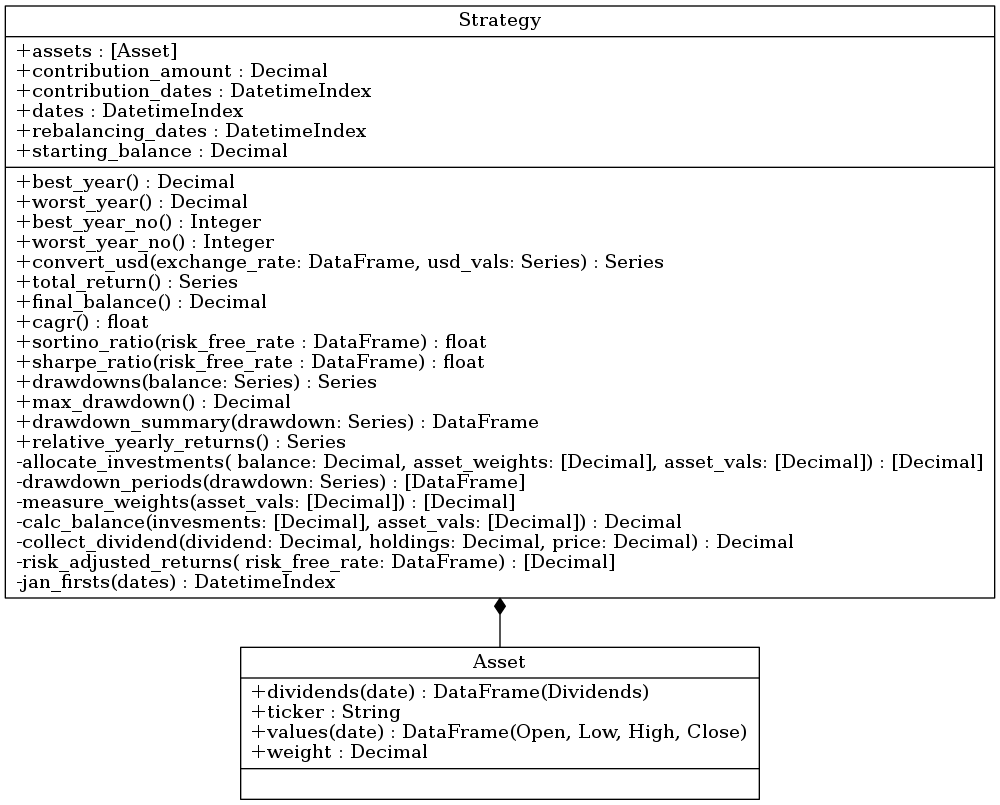
\includegraphics[scale=0.8]{Report/08Appendices/084UML/084Pictures/classes_analyse_data.png}
   \caption{UML Diagrams - Anda}
\end{figure}

\subsection{Data Harvester}

\begin{figure}[H]
   \centering
   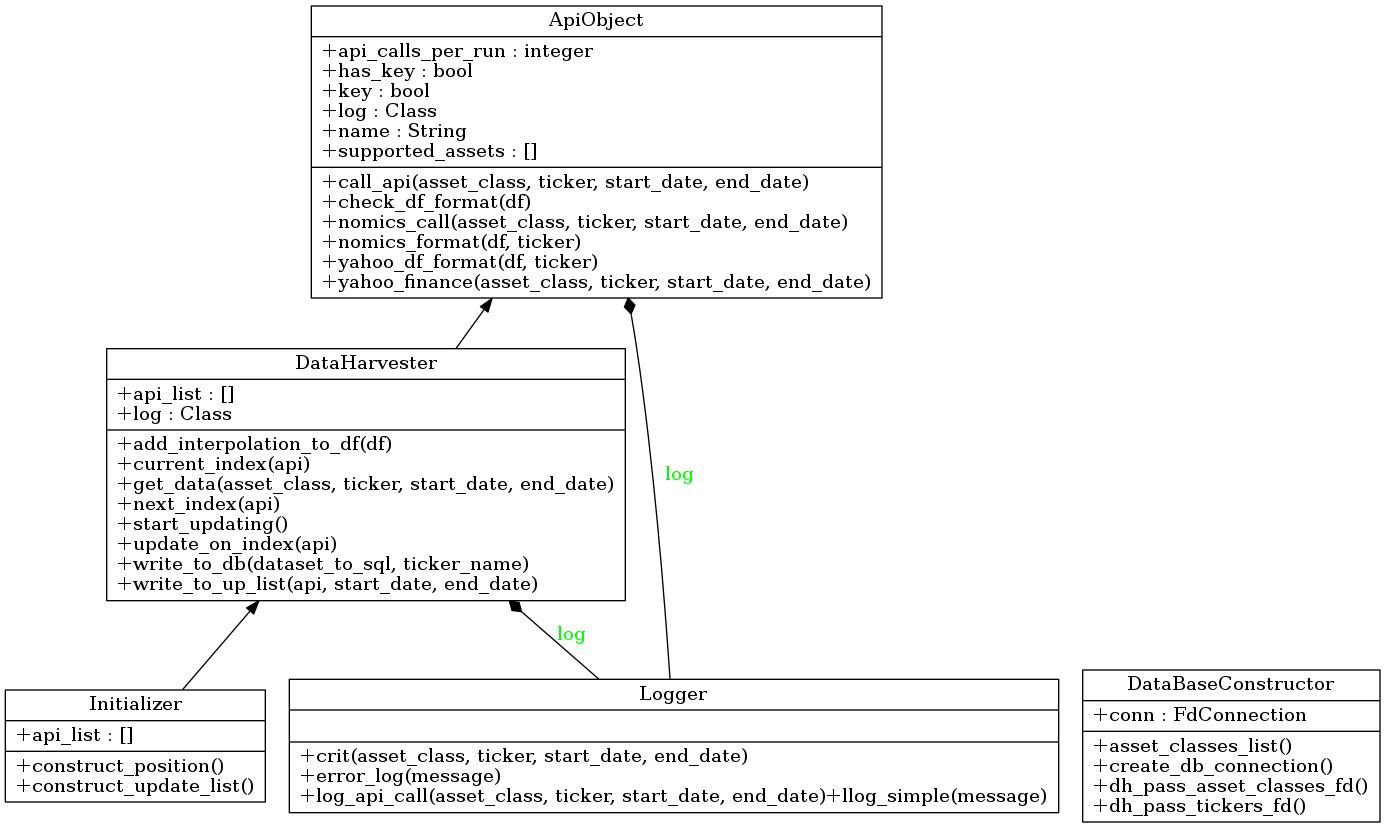
\includegraphics[scale=0.8]{Report/08Appendices/084UML/084Pictures/classes_dhav_core.png}
   \caption{UML Diagrams - Data Harvester}
\end{figure}

\subsection{Finda}

\begin{figure}[H]
   \centering
   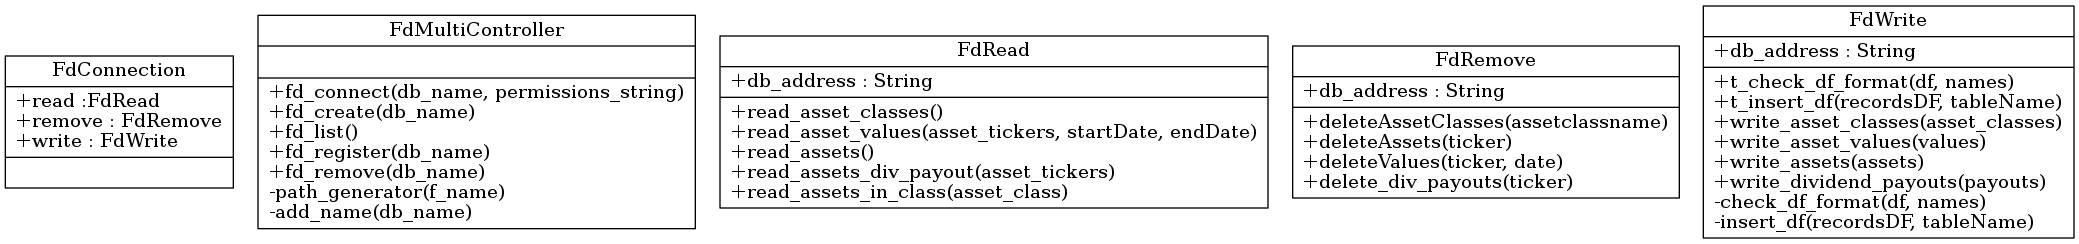
\includegraphics[scale=0.8]{Report/08Appendices/084UML/084Pictures/classes_Finda.png}
   \caption{UML Diagrams - Finda}
\end{figure}

\subsection{Thalia Web}

\begin{figure}[H]
   \centering
   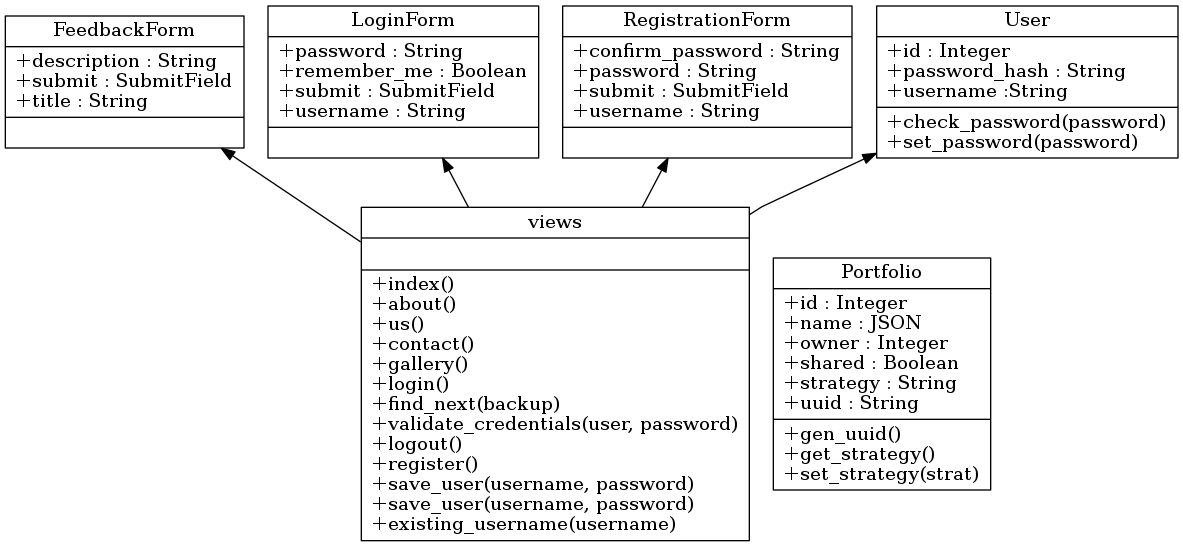
\includegraphics[scale=0.8]{Report/08Appendices/084UML/084Pictures/classes_thalia.png}
   \caption{UML Diagrams - Thalia Web}
\end{figure}

\end{document}